%!TEX program = xelatex
% Encoding: UTF8
% SEIKA 2015


% Chapter 2 Tutorials
% Section 2.4 TensorFlow Mechanics 101


\newpage
\section {TensorFlow Mechanics 101} \label{tf_mech101}

代码地址: \href{https://tensorflow/g3doc/tutorials/mnist/}{tensorflow/g3doc/tutorials/mnist/}

本篇教程的目的,是向大家展示如何利用TensorFlow使用(经典)MNIST数据集训练并评估一个用于识别手写数字的简易前馈神经网络(feed-forward neural network)。我们的目标读者是有兴趣使用TensorFlow的机器学习资深人士。

因此,撰写该系列教程并不是为了教大家机器学习领域的基础知识。

在学习本教程之前,请确保您已按照安装TensorFlow教程中的要求,完成了安装。

\subsection {教程使用的文件} \label{minist_tf}

本教程引用如下文件:

% add table here

只需要直接运行fully\_connected\_feed.py文件,就可以开始训练:

python fully\_connected\_feed.py

\subsection {准备数据}

MNIST是机器学习领域的一个经典问题,指的是让机器查看一系列大小为$28\times28$像素的手写数字灰度图像,并判断这些图像代表0--9中的哪一个数字。

\begin{figure}[htbp]
\centering

\includegraphics[width=.55\textwidth]{../SOURCE/images/MNIST.png}
\caption{}
\end{figure}

更多相关信息,请查阅Yann LeCun网站中关于MNIST的介绍 或者Chris Olah对MNIST的可视化探索。

\subsubsection{下载}

在\lstinline{run\_training()}方法的一开始,\lstinline{input\_data.read\_data\_sets()}函数会确保你的本地训练文件夹中,已经下载了正确的数据,然后将这些数据解压并返回一个含有\lstinline{DataSet}实例的字典。

\begin{lstlisting}
data_sets = input_data.read_data_sets(FLAGS.train_dir, FLAGS.fake_data)
\end{lstlisting}\footnote{\lstinline{fake_data}标记是用于单元测试的,读者可以不必理会。}

% 数据集 | 目的
% --- | ---
% `data_sets.train` | 55000个图像和标签(labels),作为主要训练集。
% `data_sets.validation` | 5000个图像和标签,用于迭代验证训练准确度。
% `data_sets.test` | 10000个图像和标签,用于最终测试训练准确度(trained accuracy)。

Add table here\footnote{了解更多数据有关信息,请查阅此系列教程的[数据下载](mnist/download/index.md)
部分.}

\subsubsection{输入与占位符}
% ### 输入与占位符(Inputs and Placeholders) <a class="md-anchor" id="AUTOGENERATED-inputs-and-placeholders"></a>

\lstinline{placeholder_inputs()}函数将生成两个\lstinline{tf.placeholder}
%[`tf.placeholder`](../api_docs/python/io_ops.md#placeholder)
操作,定义传入图表中的shape参数,shape参数中包括\lstinline{batch_size}值,后续还会将实际的训练用例传入图表。

\begin{lstlisting}
images_placeholder = tf.placeholder(tf.float32, shape=(batch_size, IMAGE_PIXELS))
labels_placeholder = tf.placeholder(tf.int32, shape=(batch_size))
\end{lstlisting}

在训练循环(training loop)的后续步骤中,传入的整个图像和标签数据集会被切片,以符合每一个操作所设置的 \lstinline{batch_size}值,占位符操作将会填补以符合这个\lstinline{batch_size}值。然后使用\lstinline{feed_dict}参数,将数据传入\lstinline{sess.run()}函数。

\subsection {构建图表 (Build the Graph)}
%## 构建图表 (Build the Graph)<a class="md-anchor" id="AUTOGENERATED-build-the-graph"></a>

在为数据创建占位符之后,就可以运行\lstinline{mnist.py}文件,经过三阶段的模式函数操作:\lstinline{inference()}, \lstinline{loss()\lstinline},和\lstinline{training()}。图表就构建完成了。

\begin{enumerate}

\item \lstinline{inference()} —— 尽可能地构建好图表,满足促使神经网络向前反馈并做出预测的要求。

\item \lstinline{loss()} —— 往inference图表中添加生成损失(loss)所需要的操作(ops)。

\item \lstinline{training()} —— 往损失图表中添加计算并应用梯度(gradients)所需的操作。
\end{enumerate}

\begin{figure}[htbp]
\centering
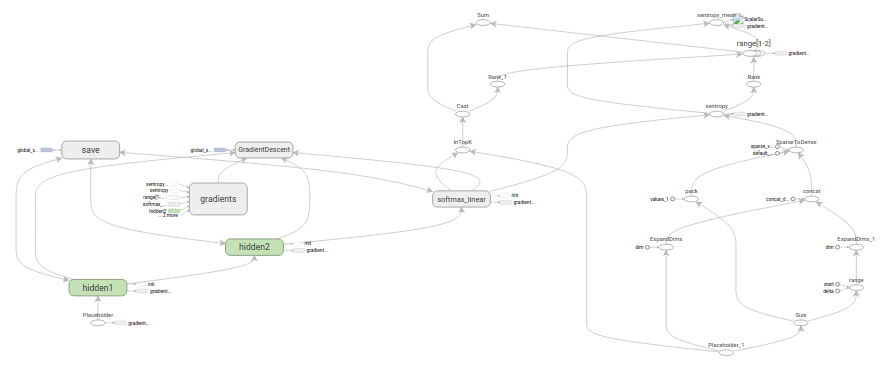
\includegraphics[width=.95\textwidth]{../SOURCE/images/mnist_subgraph.png}
\caption{}
\end{figure}

\subsubsection{推理(Inference)}
%### 推理(Inference) <a class="md-anchor" id="AUTOGENERATED-inference"></a>

\lstinline{inference()}函数会尽可能地构建图表,做到返回包含了预测结果(output prediction)的Tensor。

它接受图像占位符为输入,在此基础上借助ReLu(Rectified Linear Units)激活函数,构建一对完全连接层(layers),以及一个有着十个节点(node)、指明了输出logtis模型的线性层。

每一层都创建于一个唯一的\lstinline{tf.name_scope}%(../api_docs/python/framework.md#name_scope)
之下,创建于该作用域之下的所有元素都将带有其前缀。

\begin{lstlisting}
with tf.name_scope('hidden1') as scope:
\end{lstlisting}

在定义的作用域中,每一层所使用的权重和偏差都在\lstinline{tf.Variable}
%(../api_docs/python/state_ops.md#Variable)
实例中生成,并且包含了各自期望的shape。

\begin{lstlisting}
weights = tf.Variable(tf.truncated_normal([IMAGE_PIXELS, hidden1_units], stddev=1.0 / math.sqrt(float(IMAGE_PIXELS))), name='weights')
biases = tf.Variable(tf.zeros([hidden1_units]), name='biases')
\end{lstlisting}

例如,当这些层是在\lstinline{hidden1}作用域下生成时,赋予权重变量的独特名称将会是"\lstinline{hidden1/weights}"。

每个变量在构建时,都会获得初始化操作(initializer ops)。

在这种最常见的情况下,通过\lstinline{tf.truncated_normal}
%(../api_docs/python/constant_op.md#truncated_normal)
函数初始化权重变量,给赋予的shape则是一个二维tensor,其中第一个维度代表该层中权重变量所连接(connect from)的单元数量,第二个维度代表该层中权重变量所连接到的(connect to)单元数量。对于名叫\lstinline{hidden1}的第一层,相应的维度则是\lstinline{[IMAGE_PIXELS, hidden1_units]},因为权重变量将图像输入连接到了\lstinline{hidden1}层。\lstinline{tf.truncated_normal}初始函数将根据所得到的均值和标准差,生成一个随机分布。

然后,通过\lstinline{tf.zeros}
%(../api_docs/python/constant_op.md#zeros)
函数初始化偏差变量(biases),确保所有偏差的起始值都是0,而它们的shape则是其在该层中所接到的(connect to)单元数量。

图表的三个主要操作,分别是两个\lstinline{tf.nn.relu}
%(../api_docs/python/nn.md#relu)
操作,它们中嵌入了隐藏层所需的\lstinline{tf.matmul}
%(../api_docs/python/math_ops.md#matmul)
;以及logits模型所需的另外一个\lstinline{tf.matmul}。三者依次生成,各自的\lstinline{tf.Variable}实例则与输入占位符或下一层的输出tensor所连接。

\begin{lstlisting}
hidden1 = tf.nn.relu(tf.matmul(images, weights) + biases)
\end{lstlisting}

\begin{lstlisting}
hidden2 = tf.nn.relu(tf.matmul(hidden1, weights) + biases)
\end{lstlisting}

\begin{lstlisting}
logits = tf.matmul(hidden2, weights) + biases
\end{lstlisting}

最后,程序会返回包含了输出结果的`logits`Tensor。

\subsubsection{损失(Loss)}

\lstinline{loss()}函数通过添加所需的损失操作,进一步构建图表。

首先,\lstinline{labels_placeholer}中的值,将被编码为一个含有1-hot values的Tensor。例如,如果类标识符为“3”,那么该值就会被转换为:
\lstinline{[0, 0, 0, 1, 0, 0, 0, 0, 0, 0]}

\begin{lstlisting}
batch_size = tf.size(labels)
labels = tf.expand_dims(labels, 1)
indices = tf.expand_dims(tf.range(0, batch_size, 1), 1)
concated = tf.concat(1, [indices, labels])
onehot_labels = tf.sparse_to_dense(
    concated, tf.pack([batch_size, NUM_CLASSES]), 1.0, 0.0)
\end{lstlisting}

之后,又添加一个\lstinline{tf.nn.softmax_cross_entropy_with_logits}
%`](../api_docs/python/nn.md#softmax_cross_entropy_with_logits)
操作\footnote{交叉熵是信息理论中的概念,可以让我们描述如果基于已有事实,相信神经网络所做的推测最坏会导致什么结果。更多详情,请查阅博文《可视化信息理论》(http://colah.github.io/posts/2015-09-Visual-Information/)},用来比较\lstinline{inference()}函数与1-hot标签所输出的logits Tensor。

\begin{lstlisting}
cross_entropy = tf.nn.softmax_cross_entropy_with_logits(logits, onehot_labels, name='xentropy')
\end{lstlisting}

然后,使用\lstinline{tf.reduce_mean}
%(../api_docs/python/math_ops.md#reduce_mean)
函数,计算batch维度(第一维度)下交叉熵(cross entropy)的平均值,将将该值作为总损失。

\begin{lstlisting}
loss = tf.reduce_mean(cross_entropy, name='xentropy_mean')
\end{lstlisting}

最后,程序会返回包含了损失值的Tensor。

\subsubsection{训练}

\lstinline{training()}函数添加了通过梯度下降(gradient descent)将损失最小化所需的操作。

首先,该函数从\lstinline{loss()}函数中获取损失Tensor,将其交给\lstinline{[tf.scalar_summary]}
% ](../api_docs/python/train.md#scalar_summary)
,后者在与\lstinline{SummaryWriter}(见下文)配合使用时,可以向事件文件(events file)中生成汇总值(summary values)。在本篇教程中,每次写入汇总值时,它都会释放损失Tensor的当前值(snapshot value)。

\begin{lstlisting}
tf.scalar_summary(loss.op.name, loss)
\end{lstlisting}

接下来,我们实例化一个\lstinline{[tf.train.GradientDescentOptimizer]}
% (../api_docs/python/train.md#GradientDescentOptimizer)
,负责按照所要求的学习效率(learning rate)应用梯度下降法(gradients)。

\begin{lstlisting}
optimizer = tf.train.GradientDescentOptimizer(FLAGS.learning_rate)
\end{lstlisting}

之后,我们生成一个变量用于保存全局训练步骤(global training step)的数值,并使用\lstinline{minimize()}
% (../api_docs/python/train.md#Optimizer.minimize)
函数更新系统中的三角权重(triangle weights)、增加全局步骤的操作。根据惯例,这个操作被称为\lstinline{train_op},是TensorFlow会话(session)诱发一个完整训练步骤所必须运行的操作(见下文)。

\begin{lstlisting}
global_step = tf.Variable(0, name='global_step', trainable=False)
train_op = optimizer.minimize(loss, global_step=global_step)
\end{lstlisting}

最后,程序返回包含了训练操作(training op)输出结果的Tensor。

\subsection{训练模型}

一旦图表构建完毕,就通过\lstinline{fully_connected_feed.py}文件中的用户代码进行循环地迭代式训练和评估。

\subsubsection{图表 (The Graph)}

在\lstinline{run_training()}这个函数的一开始,是一个Python语言中的\lstinline{with}命令,这个命令表明所有已经构建的操作都要与默认的\lstinline{[`tf.Graph`]}
%(../api_docs/python/framework.md#Graph)
全局实例关联起来。

\begin{lstlisting}
with tf.Graph().as_default():
\end{lstlisting}

\lstinline{tf.Graph}实例是一系列可以作为整体执行的操作。TensorFlow的大部分场景只需要依赖默认图表一个实例即可。

利用多个图表的更加复杂的使用场景也是可能的,但是超出了本教程的范围。

\subsubsection{会话 (The Session)}

完成全部的构建准备、生成全部所需的操作之后,我们就可以创建一个\lstinline{tf.Session}
%(../api_docs/python/client.md#Session)
,用于运行图表。

\begin{lstlisting}
sess = tf.Session()
\end{lstlisting}

另外,也可以利用\lstinline{with}代码块生成\lstinline{Session},限制作用域:

\begin{lstlisting}
with tf.Session() as sess:
\end{lstlisting}

\lstinline{Session}函数中没有传入参数,表明该代码将会依附于(如果还没有创建会话,则会创建新的会话)默认的本地会话。

生成会话之后,所有\lstinline{tf.Variable}实例都会立即通过调用各自初始化操作中的\lstinline{sess.run()}
%(../api_docs/python/client.md#Session.run)
函数进行初始化。

\begin{lstlisting}
init = tf.initialize_all_variables()
sess.run(init)
\end{lstlisting}

\lstinline{sess.run()}
%(../api_docs/python/client.md#Session.run)
方法将会运行图表中与作为参数传入的操作相对应的完整子集。在初次调用时,\lstinline{init}操作只包含了变量初始化程序\lstinline{tf.group}
%(../api_docs/python/control_flow_ops.md#group)
。图表的其他部分不会在这里,而是在下面的训练循环运行。

\subsubsection{训练循环}

完成会话中变量的初始化之后,就可以开始训练了。

训练的每一步都是通过用户代码控制,而能实现有效训练的最简单循环就是:

\begin{lstlisting}
for step in xrange(max_steps):
    sess.run(train_op)
\end{lstlisting}

但是,本教程中的例子要更为复杂一点,原因是我们必须把输入的数据根据每一步的情况进行切分,以匹配之前生成的占位符。

\paragragh{向图表提}

执行每一步时,我们的代码会生成一个反馈字典(feed dictionary),其中包含对应步骤中训练所要使用的例子,这些例子的哈希键就是其所代表的占位符操作。

\lstinline{fill_feed_dict}函数会查询给定的\lstinline{DataSet},索要下一批次\lstinline{batch_size}的图像和标签,与占位符相匹配的Tensor则会包含下一批次的图像和标签。

\begin{lstlisting}
images_feed, labels_feed = data_set.next_batch(FLAGS.batch_size)
\end{lstlisting}

然后,以占位符为哈希键,创建一个Python字典对象,键值则是其代表的反馈Tensor。

\begin{lstlisting}
feed_dict = {
    images_placeholder: images_feed,
    labels_placeholder: labels_feed,
}
\end{lstlisting}

这个字典随后作为\lstinline{feed_dict}参数,传入\lstinline{sess.run()}函数中,为这一步的训练提供输入样例。

\paragragh{检查状态}

在运行\lstinline{sess.run()}函数时,要在代码中明确其需要获取的两个值:\lstinline{[train_op, loss]}。

\begin{lstlisting}
for step in xrange(FLAGS.max_steps):
    feed_dict = fill_feed_dict(data_sets.train, images_placeholder, labels_placeholder)
    _, loss_value = sess.run([train_op, loss], feed_dict=feed_dict)
\end{lstlisting}

因为要获取这两个值,\lstinline{sess.run()}会返回一个有两个元素的元组。其中每一个\lstinline{Tensor}对象,对应了返回的元组中的numpy数组,而这些数组中包含了当前这步训练中对应Tensor的值。由于\lstinline{train_op}并不会产生输出,其在返回的元祖中的对应元素就是\lstinline{None},所以会被抛弃。但是,如果模型在训练中出现偏差,\lstinline{loss} Tensor的值可能会变成\lstinline{NaN},所以我们要获取它的值,并记录下来。

假设训练一切正常,没有出现\lstinline{NaN},训练循环会每隔100个训练步骤,就打印一行简单的状态文本,告知用户当前的训练状态。

\begin{lstlisting}
if step % 100 == 0:
    print 'Step %d: loss = %.2f (%.3f sec)' % (step, loss_value, duration)
\end{lstlisting}

\paragraph{状态可视化}
为了释放\lstinline{[TensorBoard]}
%(../how_tos/summaries_and_tensorboard.md)
所使用的事件文件(events file),所有的即时数据(在这里只有一个)都要在图表构建阶段合并至一个操作(op)中。

\begin{lstlisting}
summary_op = tf.merge_all_summaries()
\end{lstlisting}

在创建好会话(session)之后,可以实例化一个\lstinline{tf.train.SummaryWriter}
% (../api_docs/python/train.md#SummaryWriter)
,用于写入包含了图表本身和即时数据具体值的事件文件。

\begin{lstlisting}
summary_writer = tf.train.SummaryWriter(FLAGS.train_dir, graph_def=sess.graph_def)
\end{lstlisting}

最后,每次运行\lstinline{summary_op}时,都会往事件文件中写入最新的即时数据,函数的输出会传入事件文件读写器(writer)的\lstinline{add_summary()}函数。。

\begin{lstlisting}
summary_str = sess.run(summary_op, feed_dict=feed_dict)
summary_writer.add_summary(summary_str, step)
\end{lstlisting}

事件文件写入完毕之后,可以就训练文件夹打开一个TensorBoard,查看即时数据的情况。

\begin{figure}[htbp]
\centering
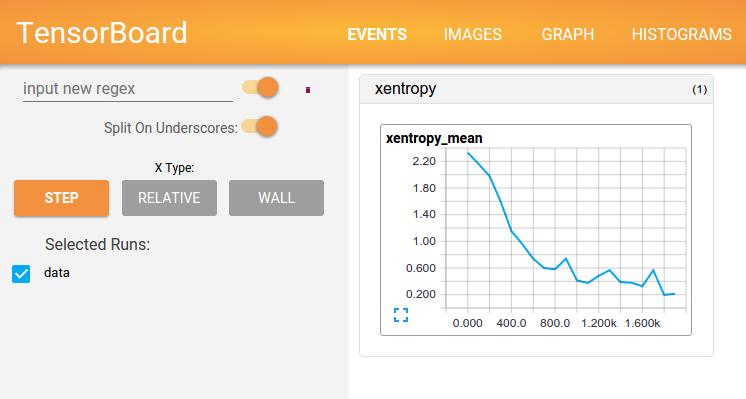
\includegraphics[width=.85\textwidth]{../SOURCE/images/mnist_tensorboard.png}
\centering
\end{figure}

% ![MNIST TensorBoard](../images/mnist_tensorboard.png "MNIST TensorBoard")

**注意**:了解更多如何构建并运行TensorBoard的信息,请查看相关教程\hyperref[vis_learning]{Tensorboard:训练过程可视化}。

\paragraph{保存检查点(checkpoint)}

为了得到可以用来后续恢复模型以进一步训练或评估的检查点文件(checkpoint file),我们实例化一个\lstinline{tf.train.Saver}
% (../api_docs/python/state_ops.md#Saver)。

\begin{lstlisting}
saver = tf.train.Saver()
\end{lstlisting}

在训练循环中,将定期调用\lstinline{saver.save()}
%(../api_docs/python/state_ops.md#Saver.save)
方法,向训练文件夹中写入包含了当前所有可训练变量值得检查点文件。

\begin{lstlisting}
saver.save(sess, FLAGS.train_dir, global_step=step)
\end{lstlisting}

这样,我们以后就可以使用\lstinline{saver.restore()}
%(../api_docs/python/state_ops.md#Saver.restore)
方法,重载模型的参数,继续训练。

\begin{lstlisting}
saver.restore(sess, FLAGS.train_dir)
\end{lstlisting}

\subsection{评估模型}

每隔一千个训练步骤,我们的代码会尝试使用训练数据集与测试数据集,对模型进行评估。\lstinline{do_eval}函数会被调用三次,分别使用训练数据集、验证数据集合测试数据集。

\begin{lstlisting}
print 'Training Data Eval:'
do_eval(sess, eval_correct, images_placeholder, labels_placeholder, data_sets.train)
print 'Validation Data Eval:'
do_eval(sess, eval_correct, images_placeholder, labels_placeholder, data_sets.validation)
print 'Test Data Eval:'
do_eval(sess, eval_correct, images_placeholder, labels_placeholder, data_sets.test)
\end{lstlisting}

>注意,更复杂的使用场景通常是,先隔绝\lstinline{data_sets.test}测试数据集,只有在大量的超参数优化调整(hyperparameter tuning)之后才进行检查。但是,由于MNIST问题比较简单,我们在这里一次性评估所有的数据。

\subsubsection {构建评估图表(Eval Graph)}

在打开默认图表(Graph)之前,我们应该先调用\lstinline{get_data(train=False)}函数,抓取测试数据集。

\begin{lstlisting}
test_all_images, test_all_labels = get_data(train=False)
\end{lstlisting}

在进入训练循环之前,我们应该先调用\lstinline{mnist.py}文件中的\lstinline{evaluation}函数,传入的logits和标签参数要与\lstinline{loss}函数的一致。这样做事为了先构建Eval操作。

\begin{lstlisting}
eval_correct = mnist.evaluation(logits, labels_placeholder)
\end{lstlisting}

\lstinline{evaluation}函数会生成\hyperref[(../api_docs/python/nn.md#in_top_k)]{\lstinline{tf.nn.in_top_k}}
操作,如果在$k$个最有可能的预测中可以发现真的标签,那么这个操作就会将模型输出标记为正确。在本文中,我们把$k$的值设置为1,也就是只有在预测是真的标签时,才判定它是正确的。

\begin{lstlisting}
eval_correct = tf.nn.in_top_k(logits, labels, 1)
\end{lstlisting}

\subsubsection {评估图表的输出(Eval Output)}

之后,我们可以创建一个循环,往其中添加\lstinline{feed_dict},并在调用\lstinline{sess.run()}函数时传入\lstinline{eval_correct}操作,目的就是用给定的数据集评估模型。

\begin{lstlisting}
for step in xrange(steps_per_epoch):
    feed_dict = fill_feed_dict(data_set,
                               images_placeholder,
                               labels_placeholder)
    true_count += sess.run(eval_correct, feed_dict=feed_dict)
\end{lstlisting}

\lstinline{true_count}变量会累加所有\lstinline{in_top_k}操作判定为正确的预测之和。接下来,只需要将正确测试的总数,除以例子总数,就可以得出准确率了。

\begin{lstlisting}
precision = float(true_count) / float(num_examples)
print '  Num examples: %d  Num correct: %d  Precision @ 1: %0.02f' % (
    num_examples, true_count, precision)
\end{lstlisting}

原文:\href{http://www.tensorflow.org/tutorials/mnist/tf/index.md}{TensorFlow Mechanics 101}
翻译:\href{https://github.com/bingjin}{bingjin}
校对:\href{https://github.com/LichAmnesia}{LichAmnesia}